%%%%%%%%%%%%%%%%%%%%%%%%%%%%%%%%%%%%%%%%%
% Beamer Presentation
% LaTeX Template
% Version 1.0 (10/11/12)
%
% This template has been downloaded from:
% http://www.LaTeXTemplates.com
%
% License:
% CC BY-NC-SA 3.0 (http://creativecommons.org/licenses/by-nc-sa/3.0/)
%
%%%%%%%%%%%%%%%%%%%%%%%%%%%%%%%%%%%%%%%%%



%\documentclass[notes]{beamer}       % print frame + notes
%\documentclass[notes=only]{beamer}   % only notes

\documentclass{beamer}
\usepackage{graphicx}% http://ctan.org/pkg/graphicx
\usepackage{pgfpages}
\usepackage{booktabs}
% These slides also contain speaker notes. You can print just the slides,
% just the notes, or both, depending on the setting below. Comment out the want
% you want.

%\setbeameroption{hide notes} % Only slides
%\setbeameroption{show only notes} % Only notes
%\setbeameroption{show notes on second screen=right} % Both


\mode<presentation> {
\usetheme{CambridgeUS}
\usecolortheme{beaver}  
}

\usepackage{graphicx} % Allows including images
\usepackage{booktabs} % Allows the use of \toprule, \midrule and \bottomrule in tables
\usepackage{booktabs}
\usepackage{moresize}
\usepackage[colorlinks]{hyperref}
\usepackage[T1]{fontenc}
\newcommand{\light}[1]{\textcolor{gray}{#1}}

%\useoutertheme{split}
%\setbeamertemplate{navigation symbols}{}

\usepackage{parskip}
\setlength{\parskip}{\smallskipamount} 

%----------------------------------------------------------------------------------------
%	TITLE PAGE
%------------------------------------------------------------------

\title [Marriage and Living Arrangement]{Parental Housing Wealth, Entry into First Marriage, and Home-leaving in Contemporary China} 

\author[Wang \& Cheng]{Donghui Wang \textsuperscript{1}  \and Cheng Cheng \inst{1,2}}

\institute [] {\textsuperscript{1} The Paul and Marcia Wythes Center on Contemporary China,      \\
                             Princeton University                                    \\
               \and  \inst{2} Center for Social Research, Peking University}  
                  
\date {August,2020}
\begin{document}
\begin{frame}
\titlepage % Print the title page as the first slide
\end{frame}





%----------------------------------------------------------------------
%	PRESENTATION SLIDES
%-----------------------------------------------------------------------


\section{Background}
\begin{frame}{Marriage Entry}
          \begin{itemize}
              \item Individual SES  
               \begin{itemize}
                   \item Education
                   \item Income, occupation
                   \item Own wealth 
               \end{itemize}
              \item Parental wealth 
               \begin{itemize}
                   \item The use value of wealth
                   \item The symbolic value of wealth 
               \end{itemize}
          \end{itemize}
\end {frame}

\begin{frame}{ Home-leaving}
          \begin{itemize}
              \item Individual SES 
          \end{itemize}
\end {frame}
          

\begin{frame}{Marriage entry and home-leaving as concurrent decisions }
\begin{itemize}
    \item Young adults consider post-marital living arrangements when making marriage decisions
    \item Most young adults remained in the parental home until marriage(Glodscheider, 1989)
    \item Late home-leaving contribute to late marriage (Raymo, 2003)
\end{itemize} 
\end {frame}

\begin{frame}{The context of China}
    \centering {Percentages of Married Individuals Living In Extended Families}
     \setlength\itemsep{1em}
    \begin{figure}
    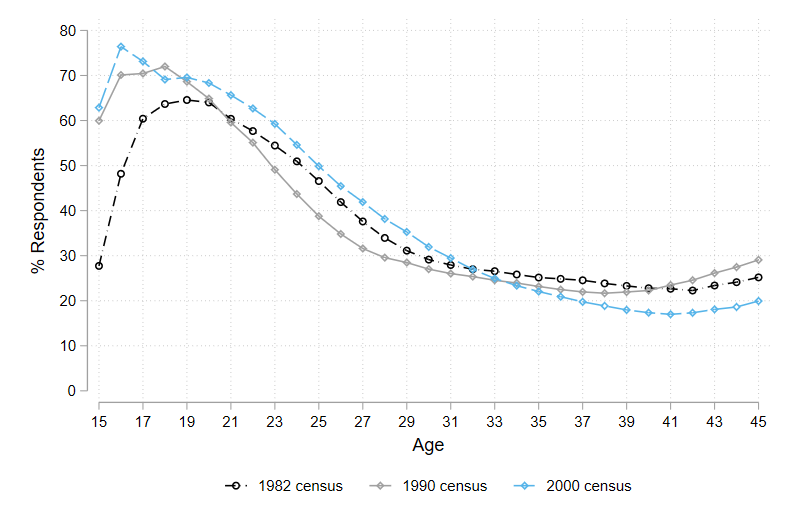
\includegraphics[width=0.9\linewidth, height=0.5\linewidth]{extended.png}
    \centering
    \end{figure}
    \tiny {Source: 1982,1990,2000 1\% micro census}
\end {frame}

\section{Research Objective}

\begin{frame}{Research Objective}
How does parental housing wealth influence children's marriage and home-leaving decisions? 
    
\end{frame}

\begin{frame}{Parental housing wealth, marriage, and home-leaving}

    
\end{frame}

% \begin{frame}{Our Approach}
% \textbf{Marriage Entry and home-leaving as concurrent decisions}
% \only<1>{
% \begin{itemize}
%     \item Young adults consider post-marital living arrangements when making marriage decisions
%     \item Most young adults remained in the parental home until marriage(Glodscheider, 1989)
%     \item Late home-leaving contribute to late marriage (Raymo, 2003)
% \end{itemize} 
% }

% \only<2>{
% Conceptualization 
% \begin{itemize}
%     \item Individuals enter marriage via two forms : Marry at natal home Vs marry outside of natal home
% \end{itemize}
% }

% \end{frame}

% \begin{frame}{Our Approach}
% \textbf{Parental housing wealth}
% \begin{itemize}
%     \item Housing wealth makes up the largest share of household wealth 
%     \item The symbolic value of housing 
% \end{itemize} 
% \end{frame}

%------------------------------------------------

%------------------------------------------------
\section{Data and Method}

\begin{frame}{}
\tableofcontents[currentsection]
\end{frame}


\begin{frame}
\frametitle{China Family Panel Studies (CFPS)}
    \begin{itemize}
            \item  Nationally representative longitudinal household survey (2010-2016)
              \begin{itemize}
              \item Track timing of marriage and change of co-residence   
                  \item Individual and family traits \textit{prior} to marriage 
              \end{itemize}
      \pause         
            \item  Analytical Sample 
            \begin{itemize}
                \item Single, age 15-45 in 2010
                \item Living with parents in 2010
                \item Final sample: 1,534 individuals (3,706 person-wave)
            \end{itemize}
    \end{itemize}

\end{frame}

\begin{frame}


\frametitle{Discrete Event History Analysis}
\begin{itemize}
    % \item Modelling waiting time; Logistic regression
    %  \pause
    \item  1. Overall rate of entry into marriage 
     \item 2.  Competing risk
       \begin{itemize}
           \item Marry at parental home 
           \item Marry outside of parental home 
       \end{itemize}

       \pause  
     \item Parental housing wealth (in logarithm form, lagged by one wave)
    
    \pause
     \item Controls 
    \begin{itemize}
       \item Own SES: Education, income (lagged by one wave)
        \item Parental SES: Education 
       \item Housing characteristics: dwelling size, if family has other property 
       \item Other characteristics : parental age, own age, if has a brother, Hukou status, if household engages farming/non-ag business 
    \end{itemize}
    

\end{itemize}

\end{frame}

%-------------------------------------
\section{Results}
\begin{frame}{Entry into marriage}
\scriptsize
\begin{table}[]
\begin{tabular}{@{}lll@{}}
\toprule
                                                                                            & M1      & M2     \\ \midrule
Housing   assets(logged)                                                                    & 0.04**   & 0.05**   \\
Parental   education                                                                        &          & -0.02    \\
Own education                                                                               &          & -0.07*** \\
Own income   (logged)                                                                       &          & 0.08***  \\
Other property                                                                              & 0.12     & 0.10     \\
\begin{tabular}[c]{@{}l@{}}Current dwelling size \\ (logged square meters)\end{tabular}     & 0.13     & 0.16*    \\
Female                                                                                      & 0.74***  & 0.87***  \\
Age spline1                                                                                 & 0.43***  & 0.40***  \\
Age spline2                                                                                 & 0.17***  & 0.14***  \\
Age spline3                                                                                 & -0.20*** & -0.23*** \\
Parental age -   individual age                                                             & -0.02    & -0.02*   \\
Han Chinese                                                                                 & 0.30     & 0.31     \\
Non-agricultural   hukou                                                                    & -0.63*** & -0.43**  \\
Has brother                                                                                 & -0.15    & -0.20    \\
Household size                                                                              & 0.03     & 0.01     \\
Household   engages in farming                                                              & 0.12     & 0.07     \\
\begin{tabular}[c]{@{}l@{}}Household   engages in \\ non-agricultural business\end{tabular} & 0.12     & 0.22     \\ \bottomrule
\end{tabular}
\end{table}
\end{frame}
%------------------------------------------------
\begin{frame}{Competing risk results}
\scriptsize

\begin{table}[]
\begin{tabular}{@{}lllll@{}}
\toprule
                                                                                            & \multicolumn{2}{l}{Marry at parental home} & \multicolumn{2}{l}{\begin{tabular}[c]{@{}l@{}}Marry outside\\  of parental home\end{tabular}} \\ \midrule
                                                                                            & M1                   & M2                  & M1                                            & M2                                            \\ \midrule
Housing   assets(logged)                                                                    & 0.06*                & 0.06*               & 0.02                                          & 0.03                                          \\
Parental   education                                                                        &                      & -0.01               &                                               & -0.03                                         \\
Own education                                                                               &                      & -0.06***            &                                               & -0.06**                                       \\
Own income   (logged)                                                                       &                      & 0.05***             &                                               & 0.09***                                       \\
Other house                                                                                 & 0.11                 & 0.09                & 0.08                                          & 0.06                                          \\
\begin{tabular}[c]{@{}l@{}}Dwelling size  \\ (logged square meters)\end{tabular}            & 0.27**               & 0.28**              & -0.05                                         & -0.03                                         \\
Female                                                                                      & -0.01                & 0.07                & 1.42***                                       & 1.57***                                       \\
Age spline1                                                                                 & 0.34***              & 0.31***             & 0.44***                                       & 0.42***                                       \\
Age spline2                                                                                 & 0.16***              & 0.15**              & 0.12*                                         & 0.09                                          \\
Age spline3                                                                                 & -0.15***             & -0.17***            & -0.23***                                      & -0.24***                                      \\
Parental age -   individual age                                                             & -0.02                & -0.02*              & -0.00                                         & -0.00                                         \\
Han Chinese                                                                                 & 0.01                 & 0.02                & 0.61*                                         & 0.62*                                         \\
Non-agricultural   hukou                                                                    & -0.49**              & -0.34               & -0.67**                                       & -0.46*                                        \\
Has brother                                                                                 & -0.51***             & -0.55***            & 0.34*                                         & 0.30*                                         \\
Household size                                                                              & -0.00                & -0.02               & 0.07                                          & 0.05                                          \\
Household   engages in farming                                                              & 0.05                 & 0.00                & 0.16                                          & 0.13                                          \\
\begin{tabular}[c]{@{}l@{}}Household   engages in \\ non-agricultural business\end{tabular} & 0.10                 & 0.17                & 0.09                                          & 0.19                                          \\ \bottomrule
\end{tabular}
\end{table}
\end{frame}



%------------------------------------------------
\begin{frame}{Recap}

\begin{itemize}
        \item Family housing wealth facilitate entry into  marriage, net of own SES 
        \item Family housing wealth facilitate marry at parental home, net of own SES 
        \item Family housing wealth do not influence marry outside of parental home 
\end{itemize}
    
\end{frame}





\begin{frame}
\Huge{\centerline{Thank you!}}
% \centerline{donghuiwang@princeton.edu}
\end{frame}

\note: household wealth reduce the risk of family division 

% \begin{frame}
% \Huge{\centerline{Additional slides}}
% % \centerline{donghuiwang@princeton.edu}
% \end{frame}

  \end{document} 
  
 